\section{Servizi di Cartografia}
Lo scopo del progetto richiede necessariamente il recupero e la manipolazione di dati cartografici, in particolare le mappe stradali e i possibili percorsi pedonali. Già dalle prime fasi del progetto, si è quindi presentata la necessità di individuare un servizio di cartografia da cui recuperare questi dati ed eventualmente sfruttare per la successiva manipolazione. I criteri di preferenza in questa scelta sono stati ancora una volta la facilità di accesso al servizio in termini di licenza, la diffusione e la documentazione disponibile.

Le due soluzioni che si sono prospettate sono i maggiori \emph{player} in questo ambito, lasciando poco spazio ad altre opzioni in termini di completezza dei dati e strumenti di integrazione. Si riassumono gli aspetti principali ed in particolare le differenze tra i due servizi che hanno determinato la scelta finale.

\subsection{Google Maps}
\begin{figure}[ht]
  \centering
  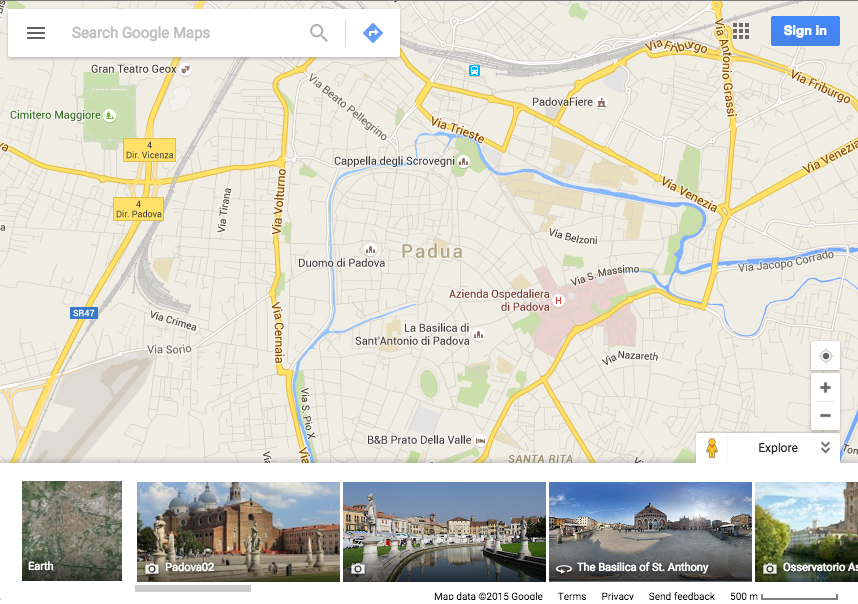
\includegraphics[width=\textwidth]{google-maps}
  \caption{\footnotesize{Schermata di accesso al servizio \emph{Google Maps}.}}
  \label{fig:google-maps}
\end{figure}
E' stato uno dei primi servizi di mappe accessibile via web, fin dall'Ottobre 2005. Negli anni si è evoluto profondamente sia in termini di completezza e accuratezza dei dati disponibli, che in termini di funzionalità e strumenti di interrogazione. Tramite Google Maps oggi è possibile accedere alle mappe stradali di tutto il mondo, percorsi pedonali, siti naturalistici, edifici pubblici di interesse, viste in prima persona e molto altro. Sono inoltre disponibili diversi strumenti per gli sviluppatori che consentono di accedere ai servizi basati su questi dati. La valutazione si è quindi concentrata sulla tipologia degli strumenti disponibili e sulle operazioni che sarebbe stato possibile eseguire (\url{https://developers.google.com/maps}).

Google fornisce \emph{API} e \emph{SDK} per le principali piattaforme applicative, sia \emph{desktop} che \emph{mobile}. Considerato però l'ambito specifico di utilizzo nel server \emph{PathS}, le funzionalità ispezionate sono quelle denominate \texttt{Web Services} ovvero interrogazioni \emph{HTTP} con risposte in formato \emph{JSON}. 

La prima caratteristica per cui si contraddistingue il servizio Google Maps è che non consente l'accesso diretto alle informazioni cartografiche. Non è possibile estrapolare parte di questi dati, siano essi in forma grezza o finita. Da qui la necessità di utilizzare uno dei servizi a disposizione per ottenere le informazioni necessarie, in particolare il servizio \textbf{Google Maps Direction API}. Con tale servizio è possibile ottenere un percorso impostando un punto di partenza ed una destinazione. Lo stesso servizio era utilizzato in precedenza dal progetto \emph{Path 2.0} e veniva impiegato direttamente per il calcolo della soluzione finale da proporre agli utenti. Tuttavia questo tipo di accesso non consente di ottenere dati per una determinata zona se non con una precisa interrogazione. Inoltre l'utilizzo delle \emph{API} presenta i seguenti limiti:
\begin{itemize}
  \item il numero di interrogazioni è limitato dal tipo di piano utilizzato. Il servizio libero e gratuito denominato \emph{Standard} consente 2,500 chiamate al giorno, applicando una tariffa per le successive. Questa situazione sarebbe stata sostenibile per le prime fasi prototipali del progetto, ma non per una sua applicazione su larga scala.
  \item il piano di utilizzo \emph{Standard} limita anche l'utilizzo della funzione ``waypoint'' nel calcolo del percorso ad 8 tappe intermedie. Questo risulterebbe un ulteriore limite nel calcolo dei percorsi complessi;
  \item il servizio Maps opera direttamente sui dati memorizzati da Google ma non è possibile aumentare o integrare direttamente questo insieme di dati. Non è possibile quindi sfruttare gli algoritmi forniti dal servizio (es. calcolo percorso) su un insieme di informazioni \emph{custom} (es. i campioni di luminosità), se non tramite un uso indiretto e improprio delle \emph{API}.
\end{itemize}
Alla data in cui si è eseguita l'analisi comparativa, i servizi \emph{Google Maps} non disponevano ancora delle \emph{Roads API} introdotte in forma sperimentale nel Marzo 2015. La funzione di interpolazione e mapping dei punti GPS sarebbe risultata molto utile all'applicazione del progetto ma per questo motivo non è stata considerata.

\subsection{OpenStreetMap}
Le mappe \emph{OpenStreetMap} (\url{http://www.openstreetmap.org}) sono il risultato di un progetto collaborativo nato nel 2004. Le informazioni cartografiche sono raccolte e corrette liberamente dai contributori la cui direzione e coordinamento sono seguiti dalla fondazione non a scopo di lucro \emph{OpenStreetMap Foundation}. Il progetto ha ormai una copertura a livello mondiale alla quale hanno contribuito sia organizzazioni governative che private tra cui ricordiamo Yahoo (2006) con le proprie ortofoto aree, l'Automotive Navigation Data (2007) con il database stradale di Paesi bassi, India e Cina ed infine l'inclusione del database stradale TIGER (2007) con le informazioni stradali degli Stati Uniti. Nel 2009 il progetto ha superato la quota dei 100.000 utenti iscritti. La caratteristica più importante dei dati \emph{OpenStreetMap} è la modalità con cui sono diffusi, ovvero coperti dalla licenza \emph{Open Database License} la quale consente un uso libero dei dati anche per prodotti derivati, purchè ne sia sempre citata la fonte originale.
Considerate le caratteristiche di libero accesso e riutilizzo, nonchè la completezza e precisione dei dati stessi, la soluzione OpenStreetMap si è candidata da subito come la soluzione ideale per l'implementazione del server \emph{PathS}. Tuttavia le modalità tecniche con cui accedere e manipolare i dati non erano immediate. Le opzioni principali offerte agli sviluppatori per consultare i dati \emph{OSM} sono (\url{http://wiki.openstreetmap.org/wiki/Develop}):
\begin{itemize}
  \item \textbf{API} (\url{http://wiki.openstreetmap.org/wiki/API_v0.6}): consentono di interrogare i dati \emph{OSM} tramite chiamate \emph{HTTP REST} e formato delle risposte \emph{XML}. Sono chiamate riservate agli \emph{editor} e non consentono di eseguire query per ampie porzioni (superiori a $0.25\deg$ quadrati).    
  \item \textbf{\emph{dump} dei dati}: ovvero estrazioni dei dati \emph{OSM} in formato \emph{XML} o come database, aggiornate in modo costante. Le estrazioni complete tuttavia hanno un volume difficilmente gestibile ($45GByte$ in formato compresso) e risulta comunque difficile accedere ad estrazioni parziali con strumenti alternativi come le API estese (\url{http://wiki.openstreetmap.org/wiki/Xapi}). 
\end{itemize}
Entrambe le opzioni non si presentano particolarmente agevoli per le esigenze del progetto, tuttavia grazie alle caratteristiche degli \emph{open data}, è stato possibile trovare delle valide alternative che, pur basandosi sui dati \emph{OSM}, fornisco modalità di integrazione più idonee al contesto.

\subsubsection{Overpass API}
Il servizio di interrogazione \emph{Overpass API} è uno strumento di introduzione recente che si è aggiunto come alternativa di consultazione in sola lettura dei dati \emph{OpenStreetMap}. Il suo scopo è quello di agire come un ``\emph{database over the web}'' che può essere interrogato in modo efficiente tramite un linguaggio specifico (\url{http://wiki.openstreetmap.org/wiki/Overpass_API}). Un client può quindi eseguire una chiamata API comunicando la \emph{query} da eseguire e in breve ottenere una risposta che raccoglie anche migliaia di elementi geografici. Il servizio è erogato liberamente e senza limitazione da infrastrutture di servizi terzi (es. \url{http://overpass-api.de}). Sono presenti inoltre strumenti on-line (ad esempio: \url{http://overpass-turbo.eu}) i quali asssitono lo sviluppo e testano l'esecuzione delle interrogazioni scritte nel formato specifico \emph{Overpass Query Language}.

\begin{figure}[ht]
  \centering
  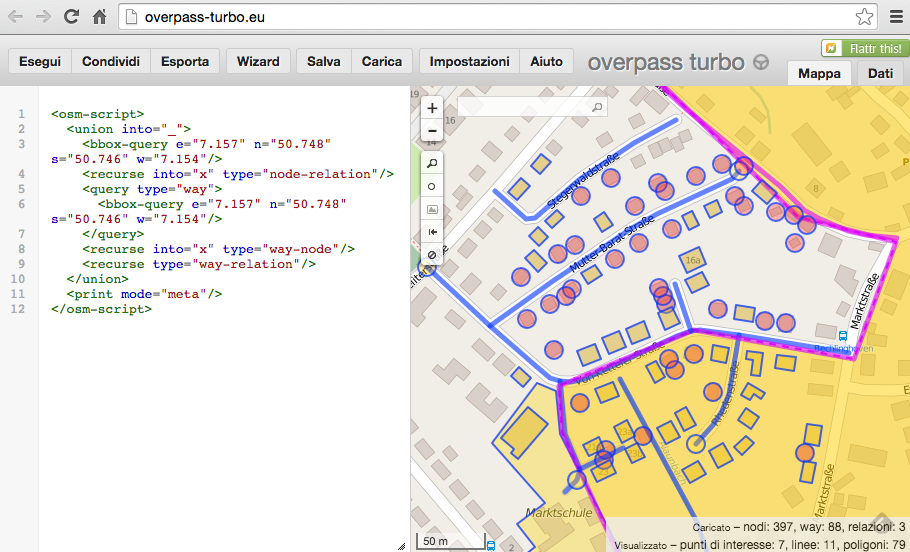
\includegraphics[width=\textwidth]{overpass}
  \caption{\footnotesize{Esempio di interrogazione tramite \emph{Overpass API}.}}
  \label{fig:overpass}
\end{figure}

Le funzionalità offerte da questa soluzione sono state valutate come ottimali nell'ambito del progetto \emph{PathS} server in quanto:
\begin{itemize}
\item sono uno strumento specificatamente sviluppato per l'integrazione lato server (\emph{webservice});
\item dispongono di sufficiente documentazione e strumenti di supporto allo sviluppo;
\item consentono di interrogare in modo parziale i dati cartografici \emph{OpenStreetMap} per la sola porzione di interesse (ad esempio il singolo percorso analizzato);
\item non impongono nessun tipo di limitazione in termini di numero o estensione delle interrogazioni.
\end{itemize}

Si è quindi studiata una \emph{query} specifica per interrogare il servizio ed ottenere i dati necessari al contesto delle elaborazioni \emph{PathS}. Per un determinato percorso o insieme di campioni ricevuti dal \emph{client}, era necessario ricavare tutti i possibili percorsi pedonali che potevano essere coinvolti. La soluzione ottenuta esegue quindi queste due operazioni:
\begin{itemize}
\item limita con una \emph{bounding box} la zona in cui eseguire l'interrogazione, ricavandola dai punti più estremi del campionamento;
\item estrae tutti i possibili elementi geografici che possono essere considerati percorsi pedonali (strade, passerelle, ponti, sentieri, etc.)
\end{itemize}
Nell'implementazione del server sono stati sviluppate alcune classi di utilità che agevolano l'interrogazione e la gestione delle risposte al servizio Overpass e sono rispettivamente: \texttt{app.\-utils.\-OverpassQuery.java} e \texttt{app.\-models.\-boundaries.\-OverpassResponse.java}.

\subsubsection{Mapquest}
Oltre al servizio di inerrogazione dei dati \emph{OpenStreetMap} si è ritenuto opportuno identificare anche un servizio di \emph{routing} che operasse sugli stessi dati, interrogabile tramite \emph{webservices} dalla componente server. Sebbene questa funzione non sia indispensabile, è risultata molto utile in fase di sviluppo e come verifica del funzionamento degli algoritmi. Il servizio è inoltre utilizzata come risposta di \emph{fallback} nel caso non vi siano dati disponibili da fornire ai \emph{client}.

La soluzione individuata è quella fornita da \emph{MapQuest} (\url{https://developer.mapquest.com}). Come per gli altri servizi, le interrogazioni avvengono tramite \emph{API HTTP} in formato \emph{JSON} e quindi gestite da alcune classi \emph{Java} di supporto per l'interrogazione (\texttt{app.\-utils.\-MapQuestQuery.java}) e l'interpretazione (\texttt{app.\-models.\-boundaries.\-MapQuestResponse.java}).


\section{Persistenza ed eleaborazione dei dati GIS}
Una delle esigenze che si presenta nello sviluppo del server \emph{PathS} è la persistenza e l'interrogazione di dati di tipo geografico. Ad esempio può essere necessario salvare le coordinate di cui si compone un percorso pedonale o ricercare tutti gli elementi salvati entro una certa distanza da una posizione nota. Per eseguire questo tipo di operazioni in modo agevole ed efficiente, è stata adottata la libreria \textbf{\emph{PostGIS}} (\url{http://postgis.net}).

Questa libreria si propone come estensione del database \emph{PostgreSQL} aggiungendo alcuni elementi fondamentali, tra cui:
\begin{itemize}
\item tipi di dato geometrico e geografico (ad esempio punti, linee spezzate, poligoni);
\item funzioni ed operatori di manipolazione dei dati geometrici (intersezione, unione, calcolo distanza, proiezione, etc.);
\item indici ed ottimizzazioni per la gestione dei dati spaziali.
\end{itemize}
Le operazioni sui dati spaziali sono acessibili come funzioni e primitive del linguaggio \emph{SQL} utilizzato per interrogare il \emph{database}. L'utilizzo di questa libreria ha consentito di implementare agevolmente le operazioni richieste dagli algoritmi e di garantire già una prima forma di ottimizzazione e accesso intelligente ai dati salvati, caratteristica non banale nel caso si fosse dovuta ri-sviluppare da zero.

Di pari passo all'odozione della libreria per il \emph{database}, si è valutata anche l'adozione di uno strumento per l'ambiente \emph{Java} il quale fornisse la rappresentazione base dei tipi geometrici le operazioni basilari su di essi. La soluzione individuata è stata la libreria \textbf{\emph{JTS}} (\url{http://www.vividsolutions.com/jts/JTSHome.htm}) la quale tramite il \emph{package} \texttt{com.\-vividsolutions.\-jts} fornisce una gerarchia di classi e operatoazioni per la rappresentazione e manipolazione di dati spaziali 2D. L'implementazione è in puro linguaggio \emph{Java} e quindi si integra facilmente nel contesto software del server.


\section{Algoritmo di Map Matching}
L'ambito a cui si applica il progetto \emph{PathS} prevede la raccolta di campioni da dispositivi che non si muovono liberamnte nello spazio ma piuttosto che seguono dei percorsi predefiniti ovvero la rete stradale e pedonale. Ottenuto un insieme di rilevamenti e le relative coordinate GPS è necessario quindi associare queste informazioni a quella che viene definita rete di trasporto. Questa associazione consente, oltre ad aumentare il contenuto informativo della base dati, ad un miglioramento e correzione dei dati relativi ai campioni, dato che o per errori nella rilevazione o per differenza di rappresentazione le coordinate potrebbero non corrispondere. 

L'operazione può essere eseguita tramite l'utilizzo di una famiglia di algoritmi denominati di \emph{Map Matching} \cite[capitolo~3.3.1]{mdme}. Tali algoritmi sono una funzione che associa a ciascuna rilevazione di un oggetto in movimento la corrispondente posizione nella rete di trasporto. 
Le tecniche di questo tipo si suddividono in due approcci:
\begin{itemize}
\item \textbf{\emph{online}}: quando i rilevamenti sono disponibili progressivamente con la loro acquisizione e spesso si applicano a contesti \emph{real-time} in cui risulta critica la velocità di risposta e i dati che si elaborano riguardano solo la situazione corrente e passata;
\item \textbf{\emph{offline}}: quando l'esecuzione dell'algoritmo può essere rimandata ad un momento successivo in cui tutte le rilevazioni sono disponibili e i vincoli temporali non sono così forti. Solitamente queste situazioni di post-processamento conducono a risultati qualitativamente migliori. 
\end{itemize}

Gli algoritmi di entrambe le categorie possono essere ulteriormente categorizzati sulla base della strategia che implementano in:
\begin{itemize}
\item \textbf{geometrici}: quando si considerano unicamente le caratteristiche geometriche dei segmenti della rete di trasporto. Alcuni esempi di questa tecnica sono gli algoritmi \emph{point-to-point}, \emph{point-to-segment} o \emph{curve-to-curve} in cui l'oggetto in movimento viene associato calcolando diversi tipi di distanza (Euclidea, perpendicolare, Fréchet).
\begin{figure}[h]
  \centering
  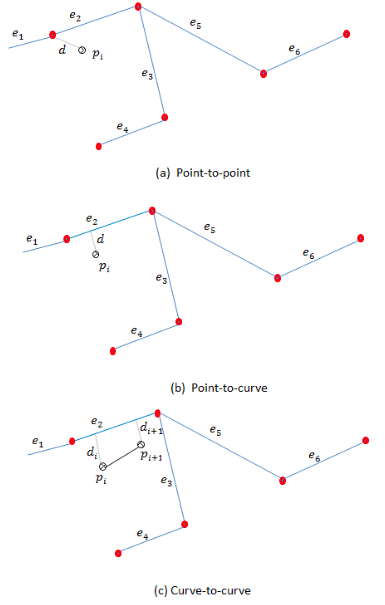
\includegraphics[width=.5\textwidth]{geometric-mapmatching}
  \caption{\footnotesize{Esempio d algoritmi di \emph{Map Matching} geometrico.}}
  \label{fig:geometric-mapmatching}
\end{figure}
\item \textbf{topologici}: quando oltre alle caratteristiche geometriche si considera anche la topologia della rete di trasporto con le possibili adiacenze e connessioni tra i vari segmenti. Generalmente questo tipo di approccio fornisce risultati migliori rispetto a quello eclusivamente geometrico ma è suscettibile di errori soprattuto in presenza di \emph{outlier}. In questa categoria non si considerano le informazioni aggiuntive come velocità e direzione del movimento. 
\item \textbf{probabilistici}: sono algoritmi che sfruttano una regione di errore, tipicamente di forma ellittica, la cui dimensione dipende dalla velocità di spostamento. Quest'area viene utilizzata per una selezione dei possibili \emph{match} in particolare nelle zone di congiunzione. La scelta finale viene eseguita considerando direzione e velocità dello spostamento, nonchè le caratteristiche di connessione degli elementi della rete.
\item \textbf{ibridi}: sono gli algoritmi che uniscono gli approcci precedenti in soluzioni particolarmente intelligenti in cui la combinazione dei vari criteri consente di eseguire scelte più accurate. Questi algoritmi inoltre possono fare uso di informazioni da sistemi terzi come ad esempio l'\emph{Assisted GPS}.
\end{itemize}

Indipendentemente dall'algoritmo utilizzato, i risultati dipendono molto dall'accuratezza della risoluzione della mappa: più alta è la definizione, migliori saranno i risultati ottenuti. Spesso gli algoritmi presuppongono che le informazioni sulla rete di trasporto siano corrette e complete. Così è anche nel progetto \emph{PathS} in cui si assume come insieme completo i dati estratti da \emph{OpenStreetMap} e i campioni vengono associati a quei percorsi. In altre situazioni tuttavia è anche possibile utilizzare gli algoritmi di \emph{Map Maptching} per l'operazione inversa, ovvero migliorare la risoluzione o estendere la rete di trasporto a partire dai rilevamenti di un oggetto in movimento. Questo aspetto non è stato considerato in questa fase di progetto ma solo come possibile evoluzione.

\subsection{ST-MapMatching}
Per l'applicazione al progetto \emph{PathS} è stato necessario individuare un algoritmo di \emph{Map Matching} che consentisse l'associazione dei rilevamenti di rumore e luminosità ai tratti di percorso delle mappe \emph{OpenStreetMap}. 

L'utilizzo di un algoritmo di tipo \emph{offline} è lecito, dato che l'elaborazione dei percorsi può avvenire dopo il loro invio alla componente \emph{server} e in quel caso tutti i rilevamenti sono stati eseguiti. Inoltre l'operazione non è direttamente collegata ad una interrogazione dell'utente ma piuttoto ad un processo \emph{batch} di elaborazione del server, il quale può tollerare anche una alta complessità computazionale e tempi di elaborazione lunghi.

Tra le alternative disponibili in letteratura, si è optato per una opzione che fosse relativamente semplice da implementare e al tempo stesso garantisse dei risultati qualitativamente accettabili. Un algoritmo di tipo esclusivamente geometrico ad esempio non sarebbe stato utile, dato che non tiene conto delle caratteristiche di sequenzialità dei percorsi pedonali che andiamo a trattare e potrebbe portare ad associazioni non corrette.

Un buon compromesso individuato è l'algoritmo \textbf{\emph{Spatio Temporal Map Matching} (ST Matching)} \cite{stmapmatching}. Nella soluzione si considerano sia le caratteristiche spaziali e topoligiche della rete di trasporto che i vincoli temporali e di velocità della traiettoria. L'algoritmo si compone principalmente di tre passaggi [\ref{fig:st-mapmatching}] in cui:
\begin{itemize}
	\item si analizzano i dati GPS e la rete di trasporto per l'identificazione dei possibili candidati;
	\item si valutano singolarmente i candidati tramite considerazioni spazio-temporali;
	\item si determina il \emph{matching} ottimale con il supporto di un grafo dei candidati.
\end{itemize}
\begin{figure}[h]
  \centering
  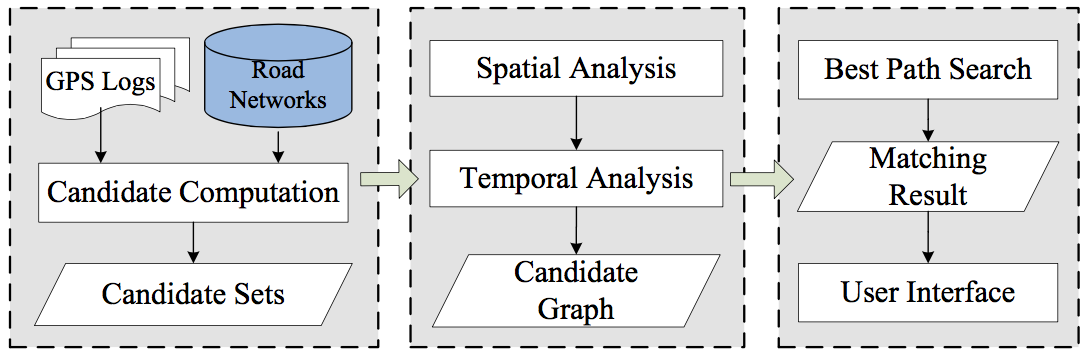
\includegraphics[width=\textwidth]{st-mapmatching}
  \caption{\footnotesize{Schema dei passi previsti dall'algoritmo \emph{ST Matching}.}}
  \label{fig:st-mapmatching}
\end{figure}
Le caratteristiche dell'algoritmo fanno si che possano ottenere dei risultati in linea con le aspettative in termini di errore di precisione e al tempo stesso delle \emph{performance} accettabili. 

Si presenta l'implemenazione di dettaglio così come è stata eseguita per ciascun passo previsto dall'algoritmo.

\subsection{Pre-elaborazione del percorso - step 1}
Il primo passo consiste nell'identificare tutti i possibili elementi della rete di trasporto che possono essere coinvolti dal percorso che si sta elaborando.

La prima operazione è quindi quella di calcolare una \emph{bounding box} in grado di contenere tutti i campioni del pecorso. Il calcolo avviene sfruttando le librerie \emph{PostGIS} e una \emph{query} opportunamente sviluppata per selezionare le cooordinate massime e minime di latitudine e longitudine per tutti i campioni GPS del percorso. I valori vengono ulteriormente allargati di un valore fisso (20 metri) per assicurarsi di coprire un'area sufficientemente estesa al netto degli errori di accuratezza.

La stessa \emph{bounding box} viene quindi utilizzata per l'interorgazione dei dati tramite \emph{OverpassAPI} e quindi si ottengono tutti i tratti della rete di trasporto possibilmente coinvolti nel percorso. Le informazioni vengono quindi inserite a database nella tabella \texttt{RoadSegment} e gestite tramite la classe di modello \texttt{app.\-models.\-RoadSegment.java}. I segmenti già presenti a sistema non vengono duplicati. 

Le operazioni citate sono implementate nel metodo \texttt{doStep1()} della classe \texttt{app.\-controllers.\-MaMatching.java} e il risultato della pre-elaborazione può essere visulazzato tramite l'apposita interfaccia del server (figura \ref{fig:st-mapmatching-step1}). La \emph{bounding box} è rappresentata in arancione, mentre tutti i segmenti verdi sono gli elementi elaborati e aggiunti a sistema.

\begin{figure}[h]
  \centering
  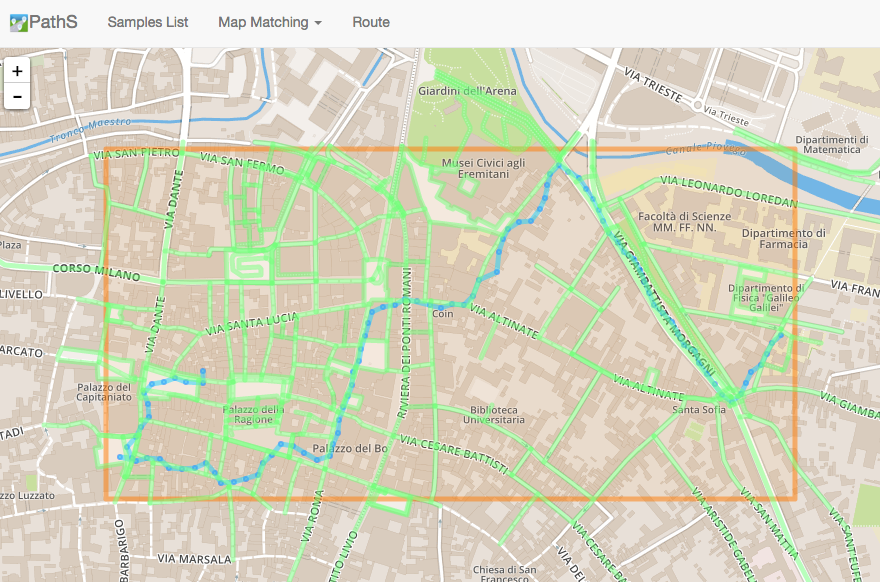
\includegraphics[width=.8\textwidth]{st-mapmatching-step1}
  \caption{\footnotesize{Risultato dell'esecuzione \emph{step} 1 dell'algoritmo \emph{ST Matching}.}}
  \label{fig:st-mapmatching-step1}
\end{figure}

\subsection{Identificazione dei candidati - step 2}
Il passo successivo dell'algoritmo è l'individuazione, per ciascun campione, dei possibili candidati. Per ciascuna posizione GPS, la quale potrebbe non appartenere alla rete di trasporto, si ricercano le possibili corrispondenze. Data quindi la traiettoria $T=p_1 \rightarrow p_2 \rightarrow ... p_n$ si ricava per ciascun punto $p_i, 1 \leq i \leq n$ i possibili segmenti candidati in un raggio $r$. Tale operazione è implementata con una \emph{query GIS} e la funzione \texttt{ST\_DWithin}. La distanza utilizzata per la selezione dei segmenti da considerare è stata impostata sperimentalmente alla misura di 20 metri. 

Per ciascun segmento vengono quindi calcolati i \textbf{punti candidati} calcolando la \emph{Line Segment Projection}. La \emph{Line Segment Projection} di un punto $p$ rispetto ad un segmento di rete di trasprot $e$ è definita come il punto $c$ appartenente ad $e$ tale per cui $c=arg\, min_{\forall c_i \in e} dist(c_i, p)$ dove $dist(c_i, p)$ ritorna la distanza di ciascun punto $c_i$ su $e$. [\ref{fig:st-mapmatching-candidates}]

\begin{figure}[h]
  \centering
  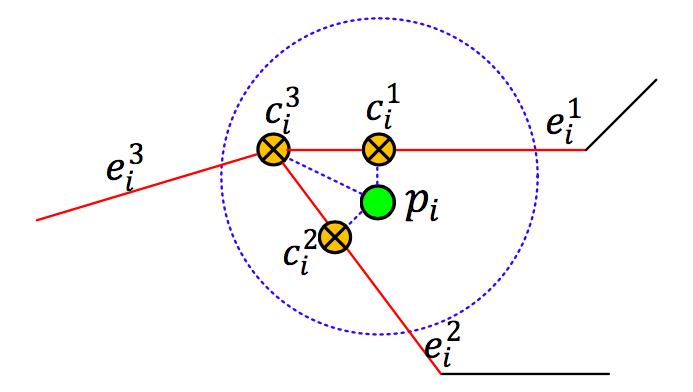
\includegraphics[width=.3\textwidth]{st-mapmatching-candidates}
  \caption{\footnotesize{Calcolo dei candidati di un punto con il metodo \emph{Line Segment Projection}.}}
  \label{fig:st-mapmatching-candidates}
\end{figure}

L'implementazione del calcolo è risultato relativamente agevole tramite la funzione \texttt{ST\_ClosestPoint(geometry, geometry)} fornita dalla libreria \emph{PostGIS}. In questo modo per ciacun punto sono state ricavate le coordinate delle proiezioni sui segmenti adiacenti e quindi possibili candidati per il \emph{matching}. I punti ottenuti sono salvati a database tramite la classe di modello \texttt{CandidatePoint}. Il risultato di questo calcolo è visualizzabile per ciascun elemento nell'interfaccia di amministrazione del server tramite i collegamenti allo \emph{step 2} (figura \ref{fig:st-mapmatching-step2}). Il punto del campionamento è indicato in colore blu mentre sono segnalate con cerchi arancioni le posizioni dei punti candidati.

\begin{figure}[h]
  \centering
  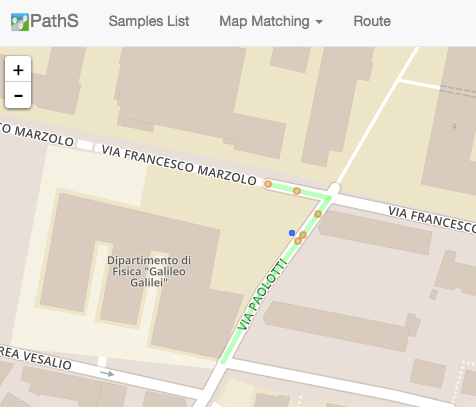
\includegraphics[width=.8\textwidth]{st-mapmatching-step2}
  \caption{\footnotesize{Risultato dell'esecuzione \emph{step} 2 dell'algoritmo \emph{ST Matching}.}}
  \label{fig:st-mapmatching-step2}
\end{figure}

Una volta individuato l'insieme dei candidati per ciascuna posizione di campionamento della traiettoria $T$, il problema si riduce a scegliere da ciascun insieme un solo elemento tale per cui: $P: c_1^j1 \rightarrow c_2^j2 \rightarrow ... c_n^jn$ è l'assegnazione ottima per $T=p_1 \rightarrow p_2 \rightarrow ... p_n$.

\subsection{Valutazione e selezione dei candidati - step 3}
Ciascun candidato viene quindi valutato considerando due aspetti:
\begin{itemize}
  \item analisi spaziale
  \item analisi temporale
\end{itemize}

Nella valutazione spaziale sono considerate sia le caratteristiche geometriche che quelle topologiche della rete di trasporto. Per ciascun punto ricavato al passo precedente vengono calcolati due valori, rispettivamente probabilità di osservazione e probabilità di trasmissione.

La prima misura indica la possibilità per cui un campione GPS $p_i$ possa coincidere con il candidato $c_i^j$ basandosi sulla distanza tra i due punti $dist(p_i, c_i^j)$. Il calcolo della probabilità si esegue assumendo che l'errore del campionamento GPS abbia una distribuzione normale con deviazione standard di 20 metri (misurazione empirica riportata in \cite[paragrafo 5.2]{stmapmatching}). Il valore della probabilità di osservazione sarà quindi tanto più elevato quanto il candidato è vicino alla posizione del campionamento. 

Tuttavia la probabilità di osservazione non tiene conto del contesto in cui si verifica la rilevazione, nè l'intorno degli altri punti. Questo può portare in diverse situazioni ad un \emph{matching} errato come quello presentato in figura \ref{fig:st-mapmatching-transmission}.

\begin{figure}[h]
  \centering
  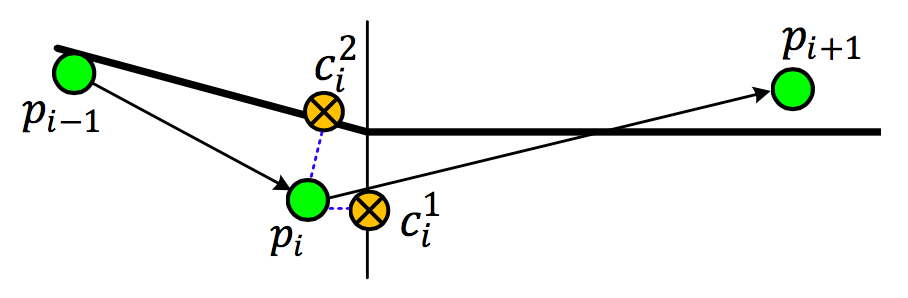
\includegraphics[width=.3\textwidth]{st-mapmatching-transmission}
  \caption{\footnotesize{Esempio di situazione in cui è necessaria la valutazione della probabilità di trasmissione.}}
  \label{fig:st-mapmatching-transmission}
\end{figure}
La linea ingrossata rappresenta una strada principale, mentre la linea più fine indica una strada secondaria. Nonostante il candidato $c_i-1$ sia più vicino al punto $p_i$ dovremma assegnare il \emph{match} al candidato $c_i^2$ in virtù del fatto che sia $p_i-1$ che $p_i+1$ sono assegnati alla strada principale. Per esprimere questa intuizione, il calcolo della probabilità di trasmissione viene eseguito rapportando la distanza euclidea tra i candidati del rilevamento precedente $c_i-1^j$ con il candidato corrente $c_i^j$ rispetto al percorso effettivo tra le due stesse posizioni seguendo il percorso più breve nella rete di trasporto (\emph{shortest path}). Tanto più questo percorso rappresenta la traiettoria ideale, tanto più alto sarà il valore dell probabilità di trasmissione.

I due valori calcolati sono quindi combinati per ottenere la valutazione totale secondo l'analisi spaziale come funzione $F_s$:
$$ F_s(c_i-1^t \rightarrow c_i^s) = N(c_i^s) * V(c_i-1^t \rightarrow c_i^s), 2 \leq i \leq n $$
dove $N$ è la funzione per il calcolo della probabilità di osservazione e $V$ è la funzione di calcolo della probabilità di trasmissione tra il candidato $c_i-1^t$ per il punto $p_i-1$ e il candidato $c_i^s$ per il punto $p_i$.

La valutazione secondo l'analisi temporale rsulta utile per i casi in cui l'analisi spaziale non sia determinante come l'esempio riportato in figura: \ref{fig:st-mapmatching-temporal}. La sola analisi geometrica non fornisce indicazioni rilevanti come invece può essere il fatto di consderare la velocità con cui si muove l'oggetto rispetto al tratto di rete di trasporto. La comparazione tra la velocità media delle rilevazioni GPS e la velocità indicativa del tratto è definita in dettaglio nel \cite[paragrafo 5.3]{stmapmatching}.
\begin{figure}[h]
  \centering
  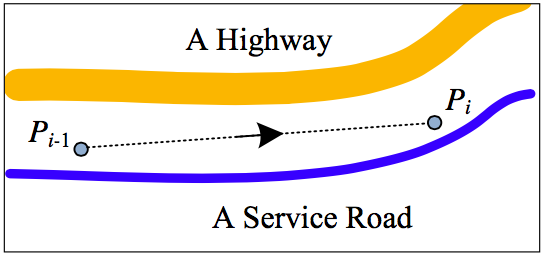
\includegraphics[width=.3\textwidth]{st-mapmatching-temporal}
  \caption{\footnotesize{Esempio di situazione in cui è necessaria l'analisi temporale.}}
  \label{fig:st-mapmatching-temporal}
\end{figure}

Tutte le operazioni di calcolo sono implementate nella classe \texttt{app.\-utils.\-STMapMatching.java} con l'ausilio della libreria matematica \emph{Apache Commons Math3}.

Eseguite l'analisi temporale e spaziale per tutti i candidati, si è in grado di generare un grafo dei candidati $G_T'(V_T', E_T')$ per la traiettoria $T=p_1 \rightarrow p_2 \rightarrow ... p_n$ in cui $V_T'$ è l'insieme dei candidati per ciascun punto di campionamento GPS ed $E_T'$ è l'insieme di tutte le connessioni tra due candidati vicini come rappresentato in figura \ref{fig:st-mapmatching-graph}.
\begin{figure}[h]
  \centering
  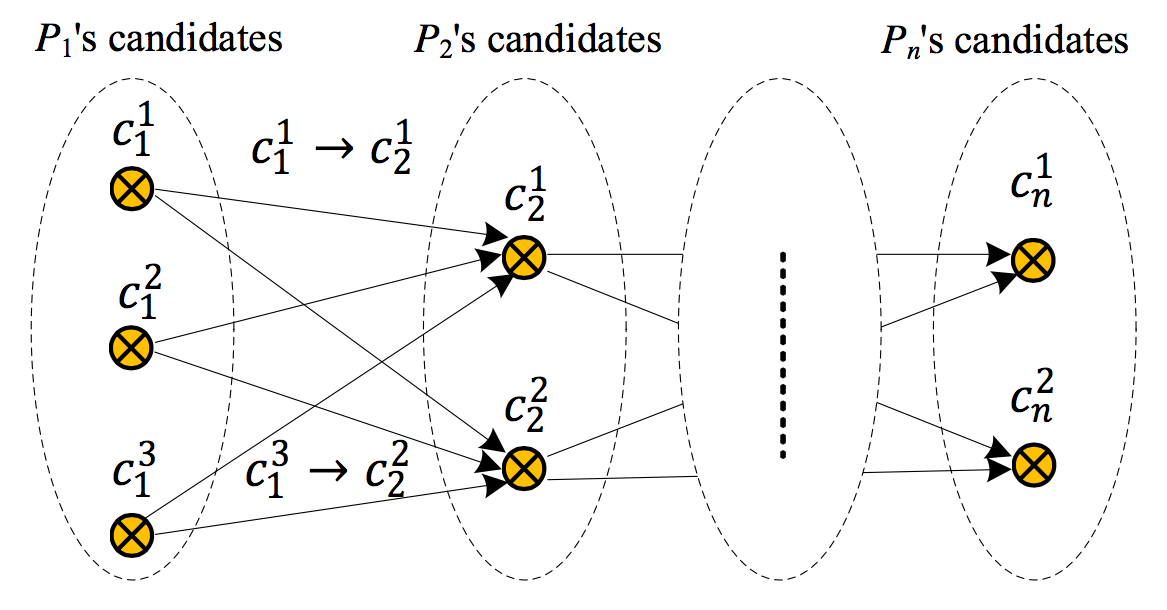
\includegraphics[width=.5\textwidth]{st-mapmatching-graph}
  \caption{\footnotesize{Grafo dei candidati.}}
  \label{fig:st-mapmatching-graph}
\end{figure}

Il problema del \emph{matching} si riconduce alla ricerca del \emph{path} di candidati $P_C$ per l'intera traiettoria $T$ definito come: $P_C: c_1^S1 \rightarrow c_1^S2 ... c_1^Sn$. Il punteggio totale per una sequenza di candidati si calcola come sommatoria delle funzioni precedentemente esposte ovvero: $F(P_C)=\sum_{i=2}^{n} F(c_i-1^{s_i-1} \rightarrow c_i^{s_i})$. Per tutti le possibili sequenze di candidati, si vuole trovare l'assegnazione ottima che copra l'intera traiettoria, espresso in termini formali:
$$P=arg max_{P_C} F(P_C), \quad \forall P_C \, \in G_T'(V_T', E_T')$$

In generale, il problema di ricerca del percorso più lungo in un grafo è \emph{NP} completo, tuttavia il fatto che il grafo sia diretto e aciclico (\emph{DAG}) fa sì che possa essere calcolato in modo efficiente sfruttando l'ordine topologico del grafico ottenuto per costruzione.

Il procedimento implementato per il calcolo è quello presentato al \cite[paragrafo 5.4]{stmapmatching}) con il nome di \emph{FindMatchedSequence} e se ne riporta lo pseudo codice.
\begin{lstlisting}[mathescape]
Input: Candidate graph $G_T'(V_T', E_T')$
Output: The longest sequence $P: c_1^s1 \rightarrow c_2^s2 \rightarrow ... c_n^sn$ in $G_T'$

Let $f[ ]$ denote the highest score computed so far;
Let $pre[ ]$ denote the parent of current candidate;

for each $c_1^s$ do
  $f[c_1^s] = N(c_1^s)$
for $i=2$ to n do
  for each $c_i^s$ do
    $max = -\infty$
    for each $c_i-1^t$ do
      $alt=f[c_i-1^t]+F(c_i-1^t \rightarrow c_i^s)$;
      if ($alt > max$) \textbf{then}
        $max = alt$
        pre[$c_i^s$] $= c_i-1^t$;
      f[$c_i^s$] $= max$;
Initialize \emph{rList} as an empty list;
$c = arg max_{c_n^s} (f[c_n^s])$
for $i=n$ to $2$ do
  rList.add(c);
  $c = pre[c]$;
rList.add(c);
return rList.reverse();
\end{lstlisting}
Il risultato dell'esecuzione dell'algortimo produce in \emph{output} il \emph{matching} ottimale per tutti i candidati. Il risultato dell'esecuzione applicato ai percorsi \emph{PathS} è consultabile da interfaccia di amministrazione tramite i collegamenti allo \emph{step 3}.

Al termine della procedura di \emph{Map Matching} il sistema interpreta i risultati ottenuti assegnando i valori dei campioni di luminosità e rumore al segmento della rete di trasporto associato. Questa informazione è considerata nelle procedure di calcolo dei percorsi presentate nel prossimo capitolo.
